\documentclass[leqno]{article}
\usepackage[utf8]{inputenc}
\usepackage{enumitem}
\usepackage{tikz}
\usepackage[parfill]{parskip} % Don't start new paragraph with tab.
\usepackage{amsmath} % For \tag and \eqref


\title{Computationele logica}
\author{
    Kamans, Jim\\
    \texttt{10302905}
    \and
    Roosingh, Sander\\
    \texttt{11983957}
    \and
    Schenk, Stefan\\
    \texttt{11881798}
}
\date{November 2017}

\begin{document}

\maketitle

\section{Exercise 1: Singapore problem}

$ \phi $ = date of Cheryl's birthday

\begin{enumerate}[label=(\alph*)]
    \item Model M of the situation immediately after Cheryl gives the boys their pieces of information: \\

    \item Epistemic sentence encoding Albert's first announcement: \\
    $ !_a (\neg K_a \phi \wedge K_a \neg K_b \phi) $

    \item Updated model M' after Albert's first announcement: \\
    \item Epistemic sentence and updated model M'' after Bernard's announcement: \\
    $ !_b (K_b \phi) $
    \item Epistemic sentence and updated model M''' after Albert's second announcement: \\
    $ !_a (K_a \phi) $
\end{enumerate}

\section{Exercise 2}
Prove formally that, for every sentence \(\varphi\), the sentence
\[\neg K_{a}\varphi \Rightarrow K_{a}\neg K_{a}\varphi\]
(expressing ``Negative Introspection of Knowledge'') is \textit{valid} on (the family of all) \textbf{epistemic} models.

Let $M = \{W, R_a, R_b, \dots, \nu\}$ be any epistemic model and let $w \in W$ be any world in it.

To prove the claim, suppose that $\neg K_a \varphi$ is true at $w$, i.e.
\begin{equation}
	\tag{1} \label{eq:ex2_1}
	w \models_M \neg K_a \varphi.
\end{equation}
We need to prove that
\begin{equation}
	\tag{?} \label{eq:ex2_?}
	w \models_M K_a \neg K_a \varphi.
\end{equation}
Let $v$ be an arbitrary world such that $w R_a v$.
By the semantics of $K_a$, \eqref{eq:ex2_1} implies


\section{Exercise 3}
Using the semantics of knowledge \(K_{a}\) and common knowledge \(Ck\), show that the following is NOT valid on \textit{epistemic models with (only) 2 agents a and b:}

\[(K_{a}K_{b}\phi\wedge K_{b}K_{a}\psi) \Rightarrow Ck(\phi\wedge\psi)\]

* = The representation of the world \\
P = $ \phi $ \\
Q = $ \psi $ \\
\\
The epistemic model holds the beliefs that both a and b know P and Q, but they are not sure whether they know the fact that both a and b know P and Q.

\begin{center}
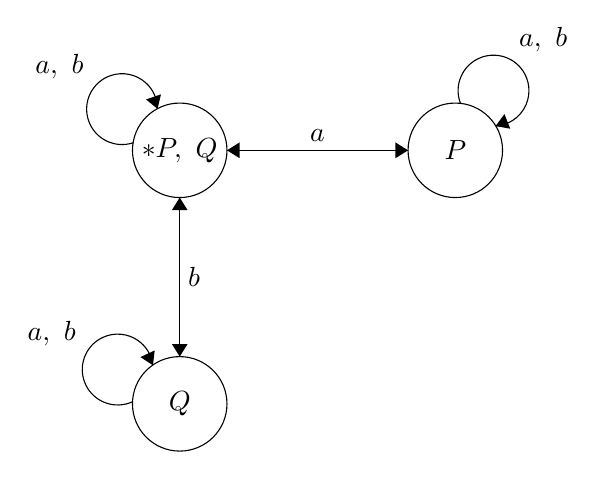
\begin{tikzpicture}[scale=0.2]
\tikzstyle{every node}+=[inner sep=0pt]
\draw [black] (13.5,-10.1) circle (3);
\draw (13.5,-10.1) node {$* P,\mbox{ }Q$};
\draw [black] (31,-10.1) circle (3);
\draw (31,-10.1) node {$P$};
\draw [black] (13.5,-26.2) circle (3);
\draw (13.5,-26.2) node {$Q$};
\draw [black] (13.5,-13.1) -- (13.5,-23.2);
\fill [black] (13.5,-23.2) -- (14,-22.4) -- (13,-22.4);
\draw [black] (16.7,-10.1) -- (28,-10.1);
\fill [black] (28,-10.1) -- (27.2,-9.6) -- (27.2,-10.6);
\draw [black] (13.5,-23.2) -- (13.5,-13.1);
\fill [black] (13.5,-13.1) -- (13,-13.9) -- (14,-13.9);
\draw (14,-18.15) node [right] {$b$};
\draw [black] (28,-10.1) -- (16.5,-10.1);
\fill [black] (16.5,-10.1) -- (17.3,-10.6) -- (17.3,-9.6);
\draw (22.25,-9.6) node [above] {$a$};
\draw [black] (10.551,-9.619) arc (288.46232:0.46232:2.25);
\draw (7.42,-4.8) node [left] {$a,\mbox{ }b$};
\fill [black] (12.09,-7.47) -- (12.31,-6.55) -- (11.36,-6.87);
\draw [black] (31.331,-7.13) arc (201.38076:-86.61924:2.25);
\draw (36.58,-3.91) node [above] {$a,\mbox{ }b$};
\fill [black] (33.56,-8.56) -- (34.49,-8.73) -- (34.12,-7.8);
\draw [black] (10.515,-26.06) arc (295.04488:7.04488:2.25);
\draw (6.93,-21.73) node [left] {$a,\mbox{ }b$};
\fill [black] (11.8,-23.75) -- (11.91,-22.81) -- (11,-23.23);
\end{tikzpicture}
\end{center}

\end{document}
